\documentclass[convert]{standalone}

\usepackage{tikz}

\tikzstyle{thickboxes}=[%
    every path/.style = {%
		darkgray, 
		line width=1pt
    },%
	myCircle/.style={%
		fill=black,
		draw=none
	}
]

\begin{document}
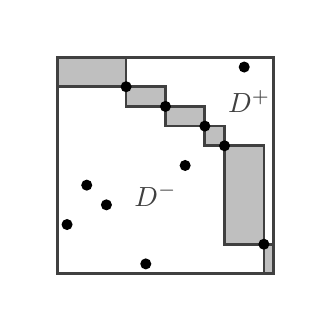
\begin{tikzpicture}[
	scale=0.25,
	baseline=(current bounding box.center),
	thickboxes
]
	\draw [draw=none, fill=white] (-1,-1) rectangle ++(14,14);
	
	\draw [fill=lightgray] (0.5,11.5) 
		|- (4,10)
		|- (6,9)
		|- (8,8)
		|- (9,7)
		|- (11,2)
		|- (11.5,0.5) 
		|- (11,2)
		|- (9,7)
		|- (8,8)
		|- (6,9)
		|- (4,10)
		|- cycle;
	\draw (0.5,0.5) rectangle ++(11,11);

	\foreach \y [count=\x] in {3, 5, 4, 10, 1, 9, 6, 8, 7, 11, 2} {
		\draw[myCircle] (\x,\y) circle (8pt);
	}

	\node at (5.5,4.5) {$D^-$};
	\node at (10.25,9.25) {$D^+$};
\end{tikzpicture}
\end{document}